\documentclass[../main/main.tex]{subfiles}


\begin{document}

\section{April  3rd, 2019}
\subsection{Shifted Inverse Power Iteration Part 2}
Let $\lambda_i,\ i=1,2,\ldots,n$ with $|\lambda_1|\le |\lambda_2|\le \ldots\le |\lambda_n|$ be eigenvalues of A. Note that $(\lambda_i-\mu)^{-1}$ are eigenvalues of $(A-\mu I)^{-1}$.\\

Thus we can apply the power iteration to $(A-\mu I)^{-1}$:
\begin{algo}
	Choose $y^{(0)}\in \R^{n}$ s.t. $\|y^{(0)}\|_2=1$\\ 
	For $k=1,2,\ldots$
	\begin{itemize}
		\item $z^{(k)}=(A-\mu I)^{-1} y^{(k-1)}$ (Done by solving $(A-\mu I)z^{(k)}=y^{(k-1)}$.
		\item $y^{(k)}=\frac{z^{(k)}}{\|z^{(k)}\|_2}$.
		\item $\mu^{(k)}=(y^{(k)})^{T}Ay^{(k)}$ (the Rayleigh Quotient of A)
	\end{itemize}
\end{algo}
\begin{enumerate}
	\item This iteration is the "shifted inverse power iteration"
	\item To make the iteration converge to $(\lambda_j,x_j)$, the following has to be satisfied:
	\begin{enumerate}
		\item $\mu$ is chosen s.t. $\frac{1}{|\lambda_j-\mu|}$ is the largest among $\frac{1}{|\lambda_i-\mu|}$
			\begin{figure}[h!]
				\centering
				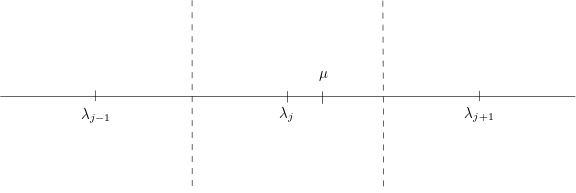
\includegraphics[width=0.8\textwidth]{4-3-choosing-mu}
				\caption{Choosing  $\mu$ to guarantee convergence}
			\end{figure}
		\item $\langle y^{(0)},x_j\rangle \neq 0$. (or else it will converge to another eigenvector.
		\item The convergence rate depends on: \[
				\frac{\frac{1}{|\lambda_j'-\mu|}}{\frac{1}{|\lambda_j-\mu|}}=\frac{|\lambda_j-\mu|}{|\lambda_j'-\mu}
		\],  where $\frac{1}{|\lambda_j'-\mu|}$ is the second largest among $\frac{1}{|\lambda_i-\mu|}$ and \[
		|\lambda_j-\mu|<|\lambda_j'-\mu|
		.\] 
	\item For an $\epsilon$- precision solution, the computational complexity is \[
	O(n^3)+O\left(\log \frac{1}{\epsilon}\cdot n^2\right)
,\] since we only compute the LU decomposition of  $\left( A-\mu I \right) $ once. 
\end{enumerate}
\end{enumerate}
To accelerate the shifted power iteration, we can also use an adaptive shift (if we shift $\mu$ to be closer to the target eigenpair, it will converge faster).
\begin{algo}[Rayleigh Quotient Iteration]
	Choose $y^{(0)}\in \R^{n}$ s.t. $\|y^{(0)}\|_2=1$\\
	$\mu^{(0)}=(y^{(0)})^{T}Ay^{(0)}$\\
	For $k=1,2,\ldots$
	\begin{itemize}
		\item $z^{(k)}=(A-\mu^{(k-1)} I)^{-1} y^{(k-1)}$ (Done by solving $(A-\mu I)z^{(k)}=y^{(k-1)}$.
		\item $y^{(k)}=\frac{z^{(k)}}{\|z^{(k)}\|_2}$.
		\item $\mu^{(k)}=(y^{(k)})^{T}Ay^{(k)}$ (the Rayleigh Quotient of A)
	\end{itemize}
	\end{algo}
i.e. we choose $\mu$ to be close to the desired eigenvalue.
\begin{itemize}
	\item This converges to some eigenpair $(\lambda_i,x_i)$ such that $\lambda_i$ is close to $\mu^{(0)}$.
	\item This Rayleigh Quotient iteration converges very fast (cubic).
\item However since $(A-\mu^{(k-1)}I)$ is changing, we have to calcualte the LU decomposition each time.
\item However, this will only converge to one eivenpair.
\end{itemize}

\subsection{Simultaneous Iteration}
To compute $r$ eigenpairs: 
\begin{algo} 
	Choose $Y^{(0)}\in R^{n\times r}$ s.t. $(Y^{(0)})^T(Y^{(0)})=I$\\
	For $k=1,2,\ldots$
	\begin{itemize}
		\item $Z^{(k)}=AY^{(k-1}$ 
		\item Set  $Y^{(k)}$ to be the Q matrix in the QR decomposition of  $Z^{(k)}$.
		\item $\mu_i^{(k)}=(y_i^{(k)})^TAy_i^{(k)}$, where $y_i^{(k)}$ is the $i$-th column of $Y^{(k)}$
	\end{itemize}
\end{algo}
	Under some assumption, we have:
	\[
		\|y_i^{(k)}-\pm x\|\le C\rho^{k}, i=1,\ldots,r
	,\] where $\rho=\max\limits_{i=1,\ldots,r}\frac{|\lambda_i+1}{\lambda_i}<1$ and $|\mu_i^{(k)}-\lambda_i|\le C\rho^k$
	\subsection{QR algorithm for Eigenvalue Decomposition}
	We set $r=n$ in the simultaneous power iteration
	\[
		Z^{(k)}=AY^{(k-1)}
	\]\[
	Y^{(k)}R^{(k)}=Z^{(k)}
,\] i.e. let $Z^{(k)}=Y^{(k)}R^{(k)}$ be the QR decomposition of $Z^{(k)}$.
Eliminating $Z^{(k)}$, we have \[
	Y^{(k)}R^{(k)}=AY^{(k-1)}\iff (Y^{(k)})^TAY^{(k-1)}=R
,\] because $(Y^{(k)})^TY^{(k)}=Y^{(k)}(Y^{(k)})^T=I$.\\

Let $A^{(k)}=(Y^{(k)})^TAY^{(k)}$, then \[
	A^{(k-1)}=(Y^{(k-1)})^TAY^{(k-1)}=(Y^{(k-1)})^TY^{(k)}R^{(k)}
.\] Since $(Y^{(k-1)})^TY^{(k)}$ is orthogonal and $R^{(k)}$ is upper triangular, $A^{(k)}$ is just an orthogonal square matrix. Note that \[
A^{(k)}=(Y^{(k)})^TAY^{(k)}=(Y^{(k)})^TAY^{(k-1)}(Y^{(k-1)})^TY^{(k)}=R^{(k)}(Y^{(k-1)})^TY^{(k)}
.\]  This means that after getting the QR decomposition of $A^{(k-1)}$, we swap the two matrices to get $A^{(k)}$.
\begin{algo}[QR Algorithm]
	Choose initial guess $A^{(0)}=(Q^{(0)})^T\forall Q^{(0)}$, e.g. $Q^{(0)}=I\implies A^{(0)}=A$.\\
	For $k=1,2,\ldots$
	\begin{itemize}
		\item Compute the QR decomposition: $A^{(k-1)}=Q^{(k)}R^{(k)}$.
		\item Set $A^{(k)}=R^{(k)}Q^{(k)}$.
	\end{itemize}
\end{algo}
\begin{remark}
	\begin{enumerate}
		\item Note that $A^{(k)}=R^{(k)}Q^{(k)}=(Q^{(k)})^{T}A^{(k-1)}Q^{(k)}$. By induction  \[
				A^{(k)}=(Q^{(k)})^T\cdots (Q^{(1)})^{T}(A^{(0)})^TAQ^{(0)}Q^{(1)}\cdots Q^{(k)}\implies A^{(k)}\text{ is similar to }A
			\] as $Q^{(0)}Q^{(1)}\cdots$ is an orthogonal matrix.
		\item Since $Y^{(k)}$ is \underline{expected} to converge to the eigenvectors of $A$, \[
				A^{(k)}=(Y^{(k)})^TAY^{(k)}\text{ is expected to converge to }\Lambda=\begin{bmatrix} \lambda_1&&\\&\ddots&\\&&\lambda_n \end{bmatrix} 
			.\] It can be proven that if the eigenvalues of $A$ are well separated, then $A^{(k)}\to \Lambda$ and $Q^{(0)}\cdots Q^{(k)}$ converges to the eigenvectors of $A$. 
		\item Since QR decomposition and matrix-matrix product costs $O(n^3)$, the total computational cost is \[
				O(kn^3),\text{ where $k$ is the number of iteration needed}
			.\] Note that if $k$ iterations is done (or if $k\sim O(n))$, then it will be $O(n^4)$, which is expensive. 
\end{enumerate}
\end{remark}
Note that even though the QR decomposition is not unique, it will still work since the QR have similar properties/structure.
\subsection{Practical Implementation of QR Algorithm}

		The idea is to choose $Q^{(0)}$ such that $A^{(0)}$ is {"well structured"}. This will allow QR decomposition to be done in $O(n^2)$. For our purpose, this "structure" is to be tridiagonal.\\
		
		Thus this implementation has two phases:
		\begin{enumerate}
			\item Find $Q^{(0)}$ such that $A^{(0)}=(Q^{(0)})^TAQ^{(0)}$ is tridiagonal.
			\item QR decomposition of tridiagonal matrices is done in $O(n^2)$ and so that $A^{(k)}$ preserves the tridiagonal structure.
		\end{enumerate}
		\begin{algo}[Phase 1]
	We will use the Householder transformation.\\
	\begin{enumerate}
		\item Let $P_1$ be the Householder transform s.t.\[
				P_1=\begin{bmatrix}1 &0&&\cdots&&0\\0&&&&&\\ &&&&&\\ \vdots&&&H_1&&\\ &&&&&\\0&&&&& \end{bmatrix} : \begin{bmatrix} 
				\times &\times & &\cdots &&\times  \\ 
				\times &\times&&\cdots&& \times \\
				&&&&&  \\
\vdots& \vdots&&\ddots&&\\
	  &&&&&\\
\times &\times&&&& \times \\
				\end{bmatrix}\to\begin{bmatrix} 
				\Delta&\Delta& &\cdots &&\Delta\\ 
				\times&\times&&\cdots&& \times \\
				0&&&&&  \\
\vdots& \vdots&&\ddots&&\\
	  &&&&&\\
0&\times&&&& \times \\
\end{bmatrix} 
		.\] Then $P_1AP_1^T$
	\end{enumerate}
\end{algo}


\end{document}

